\documentclass[tikz]{standalone}
\usepackage{pgfplots}
\pgfplotsset{compat=1.15}
\usepackage{mathrsfs}
\usetikzlibrary{arrows,calc}
\usepackage{tkz-euclide}
\pagestyle{empty}

\definecolor{AngleClr}{rgb}{0,0.39215686274509803,0}
\definecolor{ShapeClr}{rgb}{0.6,0.2,0}
\definecolor{SquareClr}{RGB}{250, 248, 217}

\begin{document}

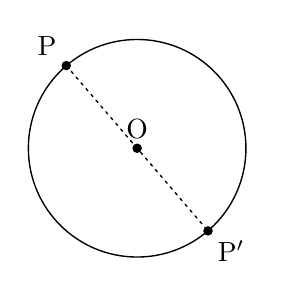
\begin{tikzpicture}[scale=.75]
\tkzSetUpLine[line width=1pt,color=black]
\tkzSetUpPoint[fill=black]

\tkzDefPoints{-1.2/1.4/P,0/0/O}

\tkzInterLC(P,O)(O,P) \tkzGetPoints{ZZ}{P'}

\tkzDrawPoints[size=3](P,O,P')

\tkzDrawSegments[line width=0.5pt,color=black,dashed,dash pattern=on 1pt off 1.75pt](P,P')

\tkzDrawCircle[line width=0.5pt,color=black](O,P)

\tkzLabelPoint[above left](P){$\rm P$}
\tkzLabelPoint[below right](P'){$\rm P'$}
\tkzLabelPoint[above](O){$\rm O$}

\end{tikzpicture}
\end{document}
